% kelompok 5 D4 TI 3B
% Restiyana Dwi Astuti (1154077)
% Boby Jamis Hari Sel (1154040)
% Rizky Abdi Perdana (1154007)
% Diki Wahyu Nugraha (1154059)
% Sabda Alamsyah (1154111)

\section{OpenGeospatialConsortium}

\subsection{Definisi}

\cite{lupp2008open} logo Open Geospatial Consortium \ref{ogc} Open Geospatial Consortium (OGC) Web Services(OWS) adalah layanan yang didefinisikan oleh OGC, yang memungkinkan semua jenis fungsi geospasial. Ini termasuk layanan untuk akses data, tampilan data dan pengolahan data. Permintaan OWS didefinisikan dengan menggunakan protokol Hyper Text Transfer Protocol (HTTP) dan dikodekan menggunakan struktur keyvalue-pair (KVP) atau Extensible Markup Language (XML). OWS yang paling banyak dikenal adalah Web Map Service (WMS).

\begin{figure}[ht]
	\centerline{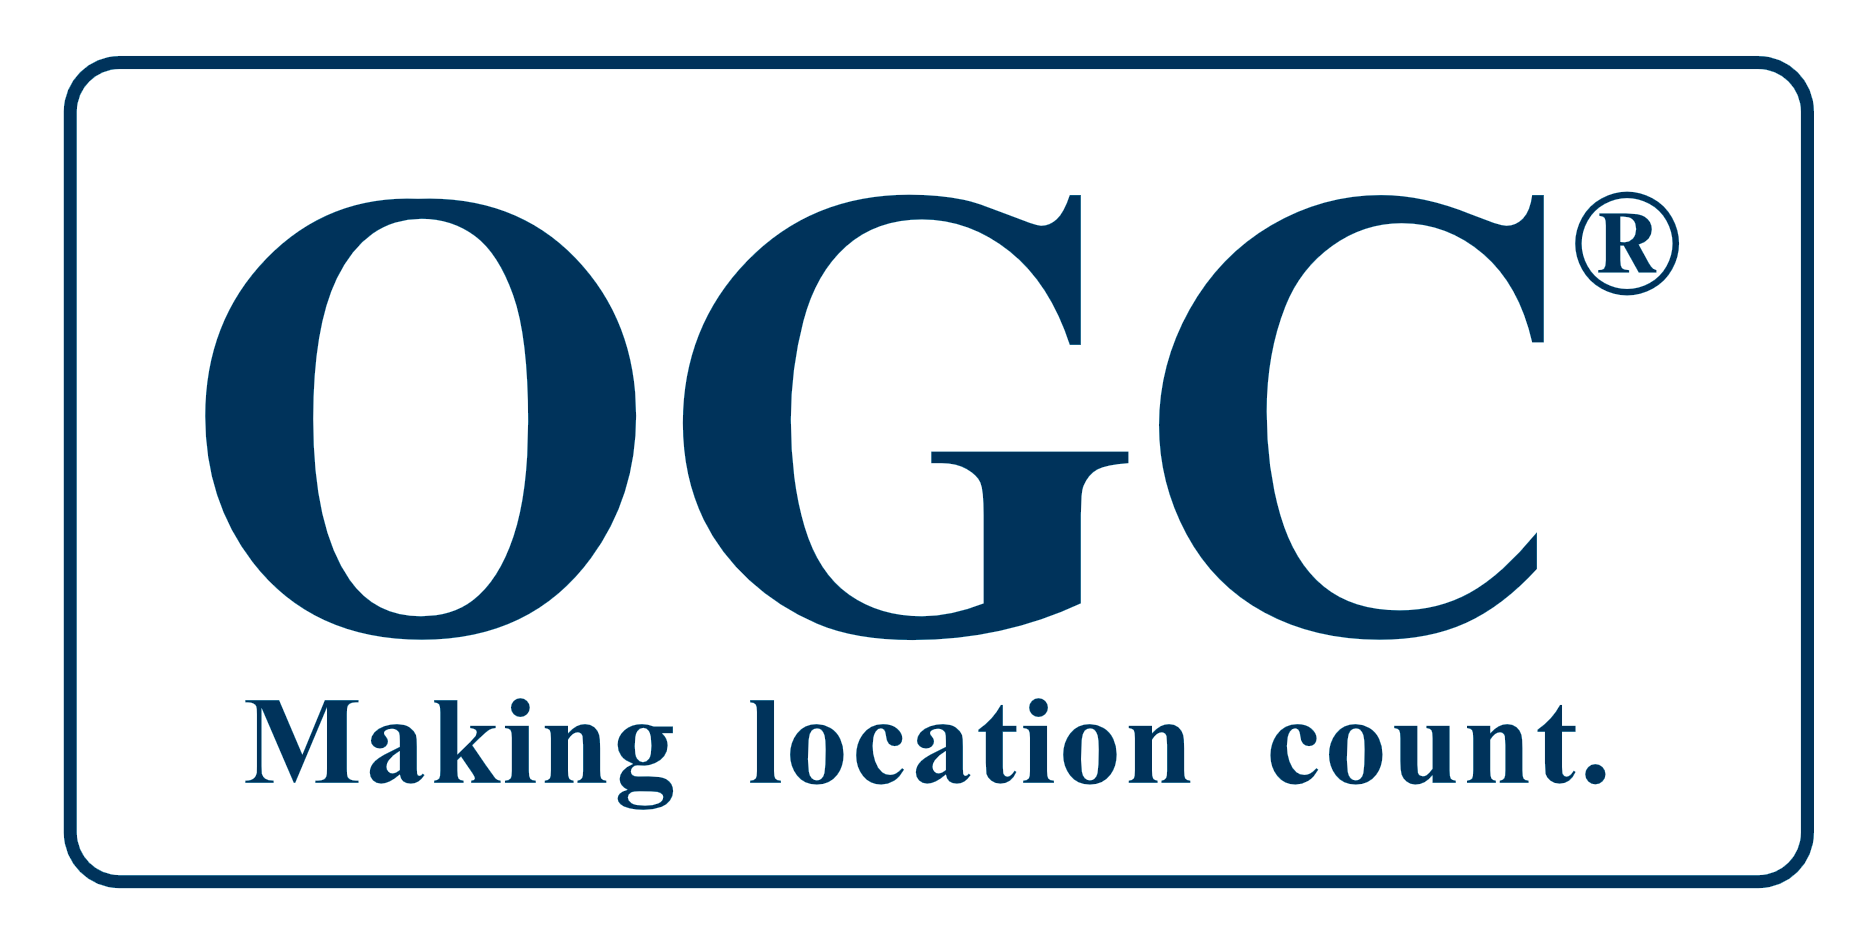
\includegraphics[width=1\textwidth]{figures/ogc.png}}
	\caption{logo}
	\label{ogc}
	\end{figure}

\subsubsection{Latar Belakang Sejarah}

\cite{lupp2008open} OGC adalah konsorsium industri internasional dari perusahaan, instansi pemerintah, organisasi penelitian, dan universitas yang berpartisipasi dalam proses konsensus untuk mengembangkan spesifikasi antarmuka yang tersedia bagi publik. Standar OpenGIS mendukung solusi interoperabilitas yang "mengaktifkan geo" layanan Web, nirkabel dan berbasis lokasi, dan arus utama TI. Pada awal 1990an, OGC mendefinisikan sebuah visi untuk komputasi geospasial berbasis jaringan. Baru-baru ini visi ini telah membuahkan hasil dengan menggunakan layanan web. Bagian ini memberikan penglihatan dari tahun 1990an diikuti oleh bagian selanjutnya yang mendefinisikan arsitektur Layanan OGC Web Services. 

Penerapan komputer dan penggunaan sistem informasi geografis (GIS) secara luas telah menyebabkan peningkatan analisis data geografis dalam banyak disiplin ilmu. Berdasarkan kemajuan teknologi informasi, ketergantungan masyarakat terhadap data tersebut semakin meningkat. Kumpulan data geografis semakin banyak dibagi, dipertukarkan, dan digunakan untuk tujuan
selain yang diinginkan produsen mereka. GIS, penginderaan jarak jauh, pemetaan otomatis dan manajemen fasilitas (AM / FM), analisis lalu lintas, sistem geopositioning, dan teknologi lainnya untuk Informasi Geografis (GI) memasuki periode integrasi radikal. 

Standar untuk interoperabilitas geospasial memberikan kerangka bagi pengembang untuk membuat perangkat lunak yang memungkinkan pengguna mengakses dan memproses data geografis dari berbagai sumber di antarmuka komputer generik dalam lingkungan teknologi informasi terbuka.
• "kerangka kerja untuk pengembang" berarti bahwa Standar Internasional didasarkan pada rencana umum yang komprehensif, umum (yaitu, dibentuk oleh konsensus untuk penggunaan umum) untuk pengembangan geoprocessing yang dapat dioperasikan.

• "akses dan proses" berarti orang-orang yang menggunakan database query remote dan mengendalikan sumber daya pemrosesan jarak jauh, dan juga memanfaatkan teknologi komputasi terdistribusi lainnya seperti perangkat lunak yang dikirim ke lingkungan lokal pengguna dari lingkungan terpencil untuk penggunaan sementara.

• "dari berbagai sumber" berarti bahwa pengguna tidak akan dapat mengakses data yang diperoleh dari berbagai cara dan disimpan dalam berbagai macam database relasional dan nonrelasional.

• "di antarmuka komputasi generik" berarti bahwa antarmuka standar menyediakan komunikasi yang andal antara sumber daya perangkat lunak yang berbeda yang dilengkapi untuk menggunakan antarmuka ini.

• "dalam lingkungan teknologi informasi yang terbuka" berarti bahwa standar memungkinkan proses geoprocessing berlangsung di luar lingkungan monolog GIS, penginderaan jarak jauh, dan AM / FM yang tertutup yang mengendalikan dan membatasi basis data, antarmuka pengguna, jaringan, dan fungsi manipulasi data.

\subsection{Dasar-dasar Ilmiah}
\cite{lupp2008open}Prinsip dasar arsitektur OGC Web Services (OWS), meliputi:

a) Komponen layanan disusun dalam beberapa tingkatan.
1. Semua komponen memberikan layanan, kepada klien dan / atau komponen lainnya, dan setiap komponen biasanya disebut layanan (dengan beberapa implementasi) atau server (masing-masing implementasi).
2. Layanan (atau komponen) diatur secara longgar dalam empat tingkatan, dari Klien sampai Layanan Aplikasi hingga Jasa Pemrosesan ke Layanan Manajemen Informasi, namun tingkat yang tidak diperlukan dapat dilewati.
3. Layanan dapat menggunakan layanan lain dalam tingkat yang sama, dan ini biasa terjadi pada tingkat Jasa Pengolahan.
4. Server dapat beroperasi pada (terikat ketat) data yang tersimpan dalam server dan / atau data (longgar terikat) yang diambil dari server lain.

b) Kolaborasi layanan menghasilkan hasil yang lebih baik.
1. Semua layanan menggambarkan diri sendiri, mendukung pengikatan layanan dinamis yang mendukung (just-in-time) yang mendukung publikasi.
2. Layanan dapat dirantai dengan layanan lain dan sering dirantai, transparan (didefinisikan dan dikendalikan oleh klien), tembus pandang (dideklarasikan tapi terlihat oleh klien), dan tidak jelas (dideklarasikan dan tidak terlihat oleh klien), lihat Sub ayat 7.3. 5 dari [ISO 19119]
3. Layanan disediakan untuk memudahkan mendefinisikan dan melaksanakan rantai layanan.

c) Komunikasi layanan menggunakan standar Internet terbuka.
1. Komunikasi antar komponen menggunakan protokol World Wide Web (WWW) standar, yaitu HTTP GET, HTTP POST, dan SOAP.
2. Operasi server khusus ditangani dengan menggunakan Uniform Resource Locators (URL).
3. Multiguna Internet Mail Extensions (MIME) jenis digunakan untuk mengidentifikasi format transfer data.
4. Data yang ditransfer sering dikodekan menggunakan Extensible Markup Language (XML), dengan isi dan format yang ditentukan menggunakan Skema XML.

d) Antarmuka layanan menggunakan standar terbuka dan relatif sederhana.
1. Antarmuka webserver OGC digabungkan, hanya memberikan beberapa operasi statis per layanan.
2. Operasi layanan biasanya tanpa kewarganegaraan, tidak memerlukan server untuk mempertahankan status antarmuka di antara operasi.
3. Satu server dapat mengimplementasikan beberapa antarmuka layanan kapanpun bermanfaat.
4. Standar pengkodean data berbasis XML XML ditentukan untuk digunakan dalam transfer data.

e) Implementasi server dan client tidak dibatasi.
1. Layanan diimplementasikan oleh perangkat lunak yang dijalankan pada komputer tujuan umum yang terhubung ke Internet. Arsitekturnya adalah perangkat keras dan vendor perangkat lunak yang netral.
2. Layanan yang sama dan bekerja sama dapat dilakukan oleh server yang dimiliki dan dioperasikan oleh organisasi independen. 
3. Banyak layanan diimplementasikan dengan software Commercial Off The Shelf (COTS) berbasis standar.

\subsection{Pengertian Geospasial} Informasi Geospasial, yang lazim dikenal dengan peta, adalah informasi
obyek permukaan bumi yang mencakup aspek waktu dan keruangan. Pengertian
geo dalam geospasial, berarti geosfer yang mencakup atmosferlapisan udara
yang meliputi permukaan bumi, litosfer lapisan kulit bumi, pedosfer tanah
beserta pembentukan dan zona-zonanya, sebagai bagian dari kulit bumi,
hidrosfer lapisan air yang menutupi permukaan bumi dalam berbagai bentuknya,
biosfer segenap unsur di permukaan bumi yang membuat kehidupan dan proses
biotik berlangsung dan antroposfer manusia dengan segala aktivitas yang
dilakukannya di permukaan bumi.

\subsubsection{Sejarah}
\cite{lupp2008open} OGC adalah konsorsium industri internasional dari perusahaan, instansi pemerintah, organisasi penelitian, 
dan universitas yang berpartisipasi dalam proses konsensus untuk mengembangkan spesifikasi antarmuka yang tersedia bagi publik. 
Standar OpenGIS mendukung solusi interoperabilitas yang "mengaktifkan geo" layanan Web, nirkabel dan berbasis lokasi, dan arus utama TI. 
Pada awal 1990an, OGC mendefinisikan sebuah visi untuk komputasi geospasial berbasis jaringan. 
Baru-baru ini visi ini telah membuahkan hasil dengan menggunakan layanan web. 
Bagian ini memberikan penglihatan dari tahun 1990an diikuti oleh bagian selanjutnya yang mendefinisikan arsitektur Layanan OGC Web Services. Penerapan komputer dan penggunaan sistem informasi geografis (GIS) secara luas telah menyebabkan peningkatan analisis data geografis dalam banyak disiplin ilmu. Berdasarkan kemajuan teknologi informasi, ketergantungan masyarakat terhadap data tersebut semakin meningkat. Kumpulan data geografis semakin banyak dibagi, dipertukarkan, dan digunakan untuk tujuan
selain yang diinginkan produsen mereka. GIS, penginderaan jarak jauh, pemetaan otomatis dan manajemen fasilitas (AM / FM), 
analisis lalu lintas, sistem geopositioning, dan teknologi lainnya untuk Informasi Geografis (GI) memasuki periode integrasi radikal.

\subsection{Definisi}
\cite{lupp2008open} Open Geospatial Consortium (OGC) Web Services(OWS) adalah layanan yang didefinisikan oleh OGC, 
yang memungkinkan semua jenis fungsi geospasial. 
Ini termasuk layanan untuk akses data, tampilan data dan pengolahan data. 
Permintaan OWS didefinisikan dengan menggunakan protokol Hyper Text Transfer Protocol (HTTP) 
dan dikodekan menggunakan struktur keyvalue-pair (KVP) atau Extensible Markup Language (XML). 
OWS yang paling banyak dikenal adalah Web Map Service (WMS).

\subsection{GeospatialWebService}
\cite{lupp2008open} Geospatial Web Service adalah jenis layanan web khusus yang menyediakan akses ke informasi geografis yang heterogen di internet ogc telah mengembangkan beberapa
spesifikasi layanan web untuk menstandardisasi layanan web geospasial untuk mengakses data dan aplikasi geospasial. 
Layanan web geospasial yang penting meliputi Web Feature Service (WFS), Web Map Service (WFS), Web Coverage Service (WCS), 
Layanan Katalog (CS), dan Web Processing Service (WPS) seperti pada gambar \ref{framework} , dll.

\begin{figure}[ht]
	\centerline{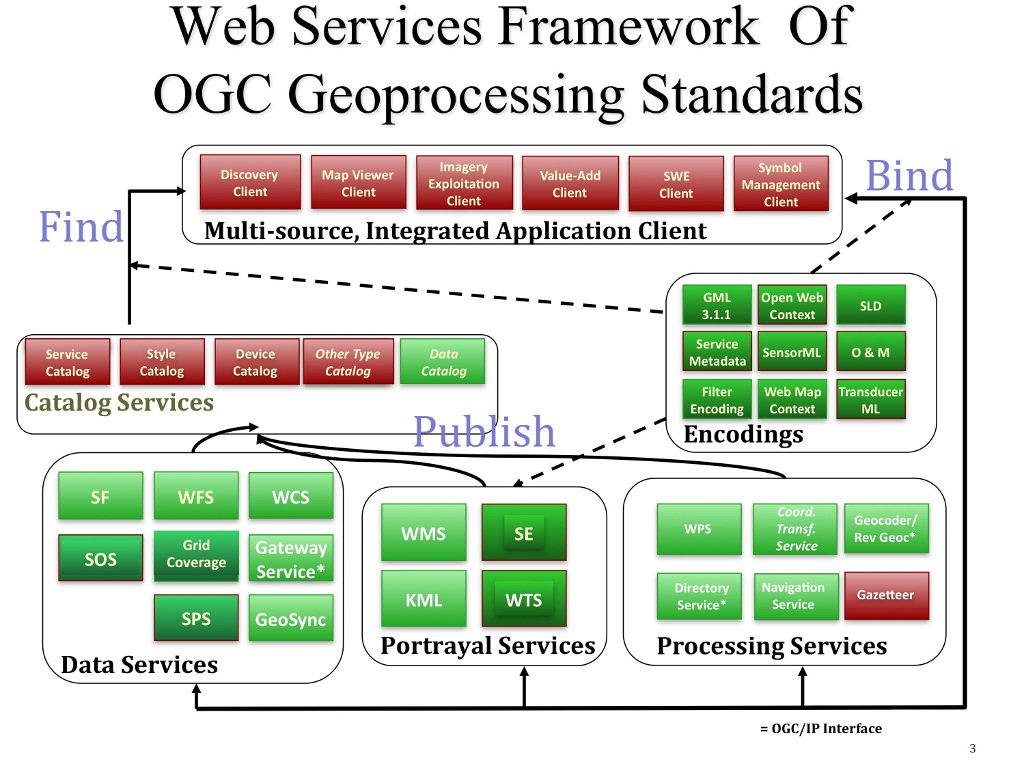
\includegraphics[width=1\textwidth]{figures/framework.JPG}}
	\caption{ogc Geoprocessing Standards}
	\label{framework}
	\end{figure}
	
\subsection{GeospatialSemanticWeb}
\cite{lupp2008open} Geospatial Semantic Web
berkaitan dengan informasi geografis bahwa penelitian semantik web dasar tidak ditujukan untuk memperbaiki 
hasil query yang mencari informasi yang tersimpan dalam database geografis.
Geospatial Semantic Web Service
alamat semantik masalah heterogen ditemukan dalam layanan web geospasial. 
layanan web semantik geospasial mendefinisikan data geospasial dan layanan pemrosesan dalam hal semantik dengan membangun 
pada entologi dan kemudian memberikan makna spesifik pada entologi tersebut

\subsection{OGC Standar}
\cite{lupp2008open} Standar OGC adalah dokumen teknis yang detail antarmuka atau pengkodean. Pengembang perangkat lunak menggunakan dokumen-dokumen ini untuk membangun antarmuka dan pengkodean yang terbuka ke dalam produk dan layanan mereka. Standar ini merupakan "produk" utama dari Konsorsium Geospasial Terbuka dan telah dikembangkan oleh anggotanya untuk mengatasi tantangan interoperabilitas yang spesifik. Idealnya, ketika standar OGC diterapkan pada produk atau layanan online oleh dua insinyur perangkat lunak yang berbeda yang bekerja secara independen, komponen dan plug and play yang dihasilkan, artinya, mereka bekerja sama tanpa melakukan debug lebih jauh.
OGC mempertahankan dua jalur standar: Jalur standar penuh dan jalur standar Komunitas. Masing-masing diringkas di bawah ini.
Jalur standar penuh: Jalur standar penuh adalah proses konsensus untuk mengembangkan dan menyetujui standar di dalam Komite Teknis OGC. Dalam jalur ini, Kelompok Kerja Standar dibuat dan kelompok tersebut menulis standar dan mendukung proses persetujuan di Panitia Teknis. Ada dua level dalam track ini:
1.	Standar OGC: ini adalah standar OGC tradisional yang menghasilkan standar yang dapat diterapkan dan dapat diuji atau model konseptual dari mana standar implementasi dapat dikembangkan; dan
2.	Standar OGC dengan Compliance Suite: ini adalah standar OGC dengan kemampuan yang telah terbukti untuk diterapkan. Untuk mencapai tingkat ini, standar OGC harus memiliki setidaknya tiga implementasi referensi dan harus ada paket uji kepatuhan Program OGC Compliance untuk semua fitur wajib standar.
Jalur standar penuh dapat menggunakan spesifikasi yang ada untuk membentuk dasar standar baru.Namun, dalam proses ini, keanggotaan OGC telah berkomitmen untuk mendukung dan mempertahankan standar melalui siklus hidupnya
Standar komunitas : standar Komunitas adalah posisi resmi OGC yang mendukung spesifikasi atau standar yang dikembangkan di luar OGC. Standar Komunitas dianggap sebagai standar normatif oleh keanggotaan OGC dan bagian dari Baseline Standar OGC. Pertimbangan utama untuk standar Komunitas adalah bahwa harus ada bukti pelaksanaan yang kuat. OGC tidak mengambil alih pemeliharaan pekerjaan, namun standar Komunitas adalah "cuplikan" dari standar matang dimana penggagas tersebut telah membagikan Hak Kekayaan Intelektual dengan OGC atau memberikan penggunaan tak terbatas atas Kekayaan Intelektual kepada semua pelaksana .
Standar masyarakat dapat melayani dua tujuan:
1.	untuk membawa standar de facto dari komunitas geospasial yang lebih besar menjadi titik acuan yang stabil yang dapat secara normatif dirujuk oleh pemerintah dan organisasi lainnya; dan
2.	untuk membawa standar baru, namun diimplementasikan, ke OGC untuk membentuk dasar bagi penyempurnaan dan pengembangan interoperabilitas lebih lanjut antara standar OGC lainnya.
Standar OGC dan dokumen pendukung tersedia untuk umum tanpa biaya apapun.
OGC Web Services (OWS) adalah standar OGC yang dibuat untuk digunakan dalam aplikasi World Wide Web.

